% Options for packages loaded elsewhere
\PassOptionsToPackage{unicode}{hyperref}
\PassOptionsToPackage{hyphens}{url}
\PassOptionsToPackage{dvipsnames,svgnames,x11names}{xcolor}
%
\documentclass[
  10pt,
  a4paper,
  twocolumn]{article}

\usepackage{amsmath,amssymb}
\usepackage{iftex}
\ifPDFTeX
  \usepackage[T1]{fontenc}
  \usepackage[utf8]{inputenc}
  \usepackage{textcomp} % provide euro and other symbols
\else % if luatex or xetex
  \usepackage{unicode-math}
  \defaultfontfeatures{Scale=MatchLowercase}
  \defaultfontfeatures[\rmfamily]{Ligatures=TeX,Scale=1}
\fi
\usepackage{lmodern}
\ifPDFTeX\else  
    % xetex/luatex font selection
\fi
% Use upquote if available, for straight quotes in verbatim environments
\IfFileExists{upquote.sty}{\usepackage{upquote}}{}
\IfFileExists{microtype.sty}{% use microtype if available
  \usepackage[]{microtype}
  \UseMicrotypeSet[protrusion]{basicmath} % disable protrusion for tt fonts
}{}
\makeatletter
\@ifundefined{KOMAClassName}{% if non-KOMA class
  \IfFileExists{parskip.sty}{%
    \usepackage{parskip}
  }{% else
    \setlength{\parindent}{0pt}
    \setlength{\parskip}{6pt plus 2pt minus 1pt}}
}{% if KOMA class
  \KOMAoptions{parskip=half}}
\makeatother
\usepackage{xcolor}
\usepackage[top=18mm,bottom=15mm,left=5mm,right=5mm]{geometry}
\ifLuaTeX
  \usepackage{luacolor}
  \usepackage[soul]{lua-ul}
\else
  \usepackage{soul}
  
\fi
\setlength{\emergencystretch}{3em} % prevent overfull lines
\setcounter{secnumdepth}{-\maxdimen} % remove section numbering
% Make \paragraph and \subparagraph free-standing
\ifx\paragraph\undefined\else
  \let\oldparagraph\paragraph
  \renewcommand{\paragraph}[1]{\oldparagraph{#1}\mbox{}}
\fi
\ifx\subparagraph\undefined\else
  \let\oldsubparagraph\subparagraph
  \renewcommand{\subparagraph}[1]{\oldsubparagraph{#1}\mbox{}}
\fi

\usepackage{color}
\usepackage{fancyvrb}
\newcommand{\VerbBar}{|}
\newcommand{\VERB}{\Verb[commandchars=\\\{\}]}
\DefineVerbatimEnvironment{Highlighting}{Verbatim}{commandchars=\\\{\}}
% Add ',fontsize=\small' for more characters per line
\newenvironment{Shaded}{}{}
\newcommand{\AlertTok}[1]{\textcolor[rgb]{1.00,0.33,0.33}{\textbf{#1}}}
\newcommand{\AnnotationTok}[1]{\textcolor[rgb]{0.42,0.45,0.49}{#1}}
\newcommand{\AttributeTok}[1]{\textcolor[rgb]{0.84,0.23,0.29}{#1}}
\newcommand{\BaseNTok}[1]{\textcolor[rgb]{0.00,0.36,0.77}{#1}}
\newcommand{\BuiltInTok}[1]{\textcolor[rgb]{0.84,0.23,0.29}{#1}}
\newcommand{\CharTok}[1]{\textcolor[rgb]{0.01,0.18,0.38}{#1}}
\newcommand{\CommentTok}[1]{\textcolor[rgb]{0.42,0.45,0.49}{#1}}
\newcommand{\CommentVarTok}[1]{\textcolor[rgb]{0.42,0.45,0.49}{#1}}
\newcommand{\ConstantTok}[1]{\textcolor[rgb]{0.00,0.36,0.77}{#1}}
\newcommand{\ControlFlowTok}[1]{\textcolor[rgb]{0.84,0.23,0.29}{#1}}
\newcommand{\DataTypeTok}[1]{\textcolor[rgb]{0.84,0.23,0.29}{#1}}
\newcommand{\DecValTok}[1]{\textcolor[rgb]{0.00,0.36,0.77}{#1}}
\newcommand{\DocumentationTok}[1]{\textcolor[rgb]{0.42,0.45,0.49}{#1}}
\newcommand{\ErrorTok}[1]{\textcolor[rgb]{1.00,0.33,0.33}{\underline{#1}}}
\newcommand{\ExtensionTok}[1]{\textcolor[rgb]{0.84,0.23,0.29}{\textbf{#1}}}
\newcommand{\FloatTok}[1]{\textcolor[rgb]{0.00,0.36,0.77}{#1}}
\newcommand{\FunctionTok}[1]{\textcolor[rgb]{0.44,0.26,0.76}{#1}}
\newcommand{\ImportTok}[1]{\textcolor[rgb]{0.01,0.18,0.38}{#1}}
\newcommand{\InformationTok}[1]{\textcolor[rgb]{0.42,0.45,0.49}{#1}}
\newcommand{\KeywordTok}[1]{\textcolor[rgb]{0.84,0.23,0.29}{#1}}
\newcommand{\NormalTok}[1]{\textcolor[rgb]{0.14,0.16,0.18}{#1}}
\newcommand{\OperatorTok}[1]{\textcolor[rgb]{0.14,0.16,0.18}{#1}}
\newcommand{\OtherTok}[1]{\textcolor[rgb]{0.44,0.26,0.76}{#1}}
\newcommand{\PreprocessorTok}[1]{\textcolor[rgb]{0.84,0.23,0.29}{#1}}
\newcommand{\RegionMarkerTok}[1]{\textcolor[rgb]{0.42,0.45,0.49}{#1}}
\newcommand{\SpecialCharTok}[1]{\textcolor[rgb]{0.00,0.36,0.77}{#1}}
\newcommand{\SpecialStringTok}[1]{\textcolor[rgb]{0.01,0.18,0.38}{#1}}
\newcommand{\StringTok}[1]{\textcolor[rgb]{0.01,0.18,0.38}{#1}}
\newcommand{\VariableTok}[1]{\textcolor[rgb]{0.89,0.38,0.04}{#1}}
\newcommand{\VerbatimStringTok}[1]{\textcolor[rgb]{0.01,0.18,0.38}{#1}}
\newcommand{\WarningTok}[1]{\textcolor[rgb]{1.00,0.33,0.33}{#1}}

\providecommand{\tightlist}{%
  \setlength{\itemsep}{0pt}\setlength{\parskip}{0pt}}\usepackage{longtable,booktabs,array}
\usepackage{calc} % for calculating minipage widths
% Correct order of tables after \paragraph or \subparagraph
\usepackage{etoolbox}
\makeatletter
\patchcmd\longtable{\par}{\if@noskipsec\mbox{}\fi\par}{}{}
\makeatother
% Allow footnotes in longtable head/foot
\IfFileExists{footnotehyper.sty}{\usepackage{footnotehyper}}{\usepackage{footnote}}
\makesavenoteenv{longtable}
\usepackage{graphicx}
\makeatletter
\def\maxwidth{\ifdim\Gin@nat@width>\linewidth\linewidth\else\Gin@nat@width\fi}
\def\maxheight{\ifdim\Gin@nat@height>\textheight\textheight\else\Gin@nat@height\fi}
\makeatother
% Scale images if necessary, so that they will not overflow the page
% margins by default, and it is still possible to overwrite the defaults
% using explicit options in \includegraphics[width, height, ...]{}
\setkeys{Gin}{width=\maxwidth,height=\maxheight,keepaspectratio}
% Set default figure placement to htbp
\makeatletter
\def\fps@figure{htbp}
\makeatother

% this merely exists to fix the loading sequence (so 'floatrow' is loaded first before 'float')
\usepackage{floatrow}
\usepackage[datesep=.]{datetime2}
\DTMsetdatestyle{ddmmyyyy}
\makeatletter
\@ifpackageloaded{tcolorbox}{}{\usepackage[skins,breakable]{tcolorbox}}
\@ifpackageloaded{fontawesome5}{}{\usepackage{fontawesome5}}
\definecolor{quarto-callout-color}{HTML}{909090}
\definecolor{quarto-callout-note-color}{HTML}{0758E5}
\definecolor{quarto-callout-important-color}{HTML}{CC1914}
\definecolor{quarto-callout-warning-color}{HTML}{EB9113}
\definecolor{quarto-callout-tip-color}{HTML}{00A047}
\definecolor{quarto-callout-caution-color}{HTML}{FC5300}
\definecolor{quarto-callout-color-frame}{HTML}{acacac}
\definecolor{quarto-callout-note-color-frame}{HTML}{4582ec}
\definecolor{quarto-callout-important-color-frame}{HTML}{d9534f}
\definecolor{quarto-callout-warning-color-frame}{HTML}{f0ad4e}
\definecolor{quarto-callout-tip-color-frame}{HTML}{02b875}
\definecolor{quarto-callout-caution-color-frame}{HTML}{fd7e14}
\makeatother
\makeatletter
\@ifpackageloaded{caption}{}{\usepackage{caption}}
\AtBeginDocument{%
\ifdefined\contentsname
  \renewcommand*\contentsname{Inhaltsverzeichnis}
\else
  \newcommand\contentsname{Inhaltsverzeichnis}
\fi
\ifdefined\listfigurename
  \renewcommand*\listfigurename{Abbildungsverzeichnis}
\else
  \newcommand\listfigurename{Abbildungsverzeichnis}
\fi
\ifdefined\listtablename
  \renewcommand*\listtablename{Tabellenverzeichnis}
\else
  \newcommand\listtablename{Tabellenverzeichnis}
\fi
\ifdefined\figurename
  \renewcommand*\figurename{Abbildung}
\else
  \newcommand\figurename{Abbildung}
\fi
\ifdefined\tablename
  \renewcommand*\tablename{Tabelle}
\else
  \newcommand\tablename{Tabelle}
\fi
}
\@ifpackageloaded{float}{}{\usepackage{float}}
\floatstyle{ruled}
\@ifundefined{c@chapter}{\newfloat{codelisting}{h}{lop}}{\newfloat{codelisting}{h}{lop}[chapter]}
\floatname{codelisting}{Listing}
\newcommand*\listoflistings{\listof{codelisting}{Listingverzeichnis}}
\makeatother
\makeatletter
\makeatother
\makeatletter
\@ifpackageloaded{caption}{}{\usepackage{caption}}
\@ifpackageloaded{subcaption}{}{\usepackage{subcaption}}
\makeatother
\makeatletter
\@ifpackageloaded{tcolorbox}{}{\usepackage[skins,breakable]{tcolorbox}}
\makeatother
\makeatletter
\@ifundefined{shadecolor}{\definecolor{shadecolor}{rgb}{.97, .97, .97}}{}
\makeatother
\makeatletter
\@ifundefined{codebgcolor}{\definecolor{codebgcolor}{HTML}{f7f7f7}}{}
\makeatother
\makeatletter
\ifdefined\Shaded\renewenvironment{Shaded}{\begin{tcolorbox}[enhanced, frame hidden, colback={codebgcolor}, breakable, sharp corners, boxrule=0pt]}{\end{tcolorbox}}\fi
\makeatother
\ifLuaTeX
\usepackage[bidi=basic]{babel}
\else
\usepackage[bidi=default]{babel}
\fi
\babelprovide[main,import]{nswissgerman}
% get rid of language-specific shorthands (see #6817):
\let\LanguageShortHands\languageshorthands
\def\languageshorthands#1{}
\ifLuaTeX
  \usepackage{selnolig}  % disable illegal ligatures
\fi
\usepackage{bookmark}

\IfFileExists{xurl.sty}{\usepackage{xurl}}{} % add URL line breaks if available
\urlstyle{same} % disable monospaced font for URLs
\hypersetup{
  pdftitle={Advanced System Design},
  pdfauthor={Joel von Rotz},
  pdflang={de-CH},
  colorlinks=true,
  linkcolor={blue},
  filecolor={Maroon},
  citecolor={Blue},
  urlcolor={Blue},
  pdfcreator={LaTeX via pandoc}}


% [GENERAL PACKAGES] ------------------------------------------------------------------- %
% includes some neato math environments, symbols and stuff
\usepackage{amssymb, amsmath}

% correctly encodes the formatting of the text files (since we live in the future of UTF8)
\usepackage[utf8]{inputenc} 

% Used for the page counter in the footer to see the amount of pages 
\usepackage{lastpage} 

% Mostly used for the titlepage. Compared to the 'twocolumn' mode, multicols allows for
% more flexible changing (without inserting newpage between column mode changes)
\usepackage{multicol}
\setlength\columnsep{20pt}

% Package for enabling colors (colorful output)
\usepackage[dvipsnames]{xcolor}
\definecolor{colorAccent}{HTML}{124E82}

% Icons - http://mirrors.ctan.org/fonts/fontawesome5/doc/fontawesome5.pdf
% This one is neat, when you want to add some icons
\usepackage{fontawesome5}

% Depending on the type of document, mostly summaries, I remove the spacing Display-styled Equations insert, since it's a waste of space.
\usepackage[nodisplayskipstretch]{setspace}

% [FONT CONFIGURATION] ----------------------------------------------------------------- %
% change the fonts here (depending which latex engine is used, this might need to be
% removed)

\usepackage{AlegreyaSans}
\usepackage{cmbright}
\usepackage[scaled=0.95]{inconsolata}

% \usepackage{AlegreyaSans}
% \usepackage{cmbright}
% \usepackage[scaled=0.95]{inconsolata} % for code blocks

% [TIKZ CONFIGURATION] ----------------------------------------------------------------- %
% Tikz is really good at creating nice looking and clean drawings, diagramms, etc. 
\usepackage{tikz}
\usetikzlibrary{shapes,arrows,arrows.meta,matrix,decorations.pathmorphing}
\newcommand*\circled[1]{\tikz[baseline=(char.base)]{
            \node[shape=circle,draw,inner sep=2pt] (char) {#1};}}           

% TIP: use 'TikzEdt' (http://www.tikzedt.org/) to preview the drawings.

% [HEADING/SECTION STYLE CONFIGURATION] ------------------------------------------------ %
% 'sectsty' is used for minor adjustments and is used to apply the bold sans serif style
% to all sections (sec, subsec, subsubsec, ...)
\usepackage{sectsty}
\allsectionsfont{\normalfont\bfseries\sffamily}

% 'titlesec' is used to customize the numbered and unnumbered sections styles (but can
% also be used for the other section types).
% 'xhfill' is used to add a ruler, centered to the text.
\usepackage{xhfill}
\usepackage[explicit]{titlesec}

\makeatletter
\newcommand \Cdotfill {\leavevmode\cleaders\hb@xt@.25em{\hss$\cdot$\hss}\hfill\kern\z@}
\makeatother

% NUMBERED - SECTIION
\titleformat
  {\section} % {⟨command⟩}
  [hang] % [⟨shape⟩]
  {\normalfont\LARGE\bfseries\filright\sffamily} % {⟨format⟩}
  {\thesection} % {⟨label⟩}
  {3mm} % {⟨sep⟩}
  {%
    \color{colorAccent}{#1\hspace{2mm}\xrfill[0.6ex]{1pt}}
  } % {⟨before-code⟩}

\titlespacing*{\section} % ⟨command⟩
  {0em} % ⟨left⟩
  {12pt} % ⟨before-sep⟩
  {6pt} % ⟨after-sep⟩

% NUMBERLESS - SECTION
\titleformat
  {name=\section,numberless} % {⟨command⟩}
  [hang] % [⟨shape⟩]
  {\normalfont\LARGE\bfseries\filright\sffamily} % {⟨format⟩}
  {} % {⟨label⟩}
  {0mm} % {⟨sep⟩}
  {%
    \color{colorAccent}{#1\hspace{2mm}}\xrfill[0.6ex]{1.2pt}[colorAccent]
  }% {⟨before-code⟩}

% NUMBERED - SUBSECTION
\titleformat{\subsection} % {⟨command⟩}
  [hang] % [⟨shape⟩]
  {\normalfont\Large\bfseries\filright\sffamily} % {⟨format⟩}
  {\thesection} % {⟨label⟩}
  {2mm} % {⟨sep⟩}
  {%
    {#1\hspace{1mm}\color{colorAccent}{\Cdotfill}}%
  } % {⟨before-code⟩}

% NUMBERLESS - SUBSECTION
\titleformat{name=\subsection,numberless} % {⟨command⟩}
  [hang] % [⟨shape⟩]
  {\normalfont\Large\bfseries\filright\sffamily} % {⟨format⟩}
  {} % {⟨label⟩}
  {0mm} % {⟨sep⟩}
  {%
    {#1\hspace{1mm}\color{colorAccent}{\Cdotfill}}%
  }% {⟨before-code⟩}

\titlespacing*{\subsection} % <command>
  {0em} % <left>
  {.5em} % <before-sep>
  {.4em} % <after-sep>

% NUMBERED - SUBSUBSECTION
\titleformat{\subsubsection} % {⟨command⟩}
  [hang] % [⟨shape⟩]
  {\normalfont\large\bfseries\sffamily} % {⟨format⟩}
  {\thesection} % {⟨label⟩}
  {2mm} % {⟨sep⟩}
  {
    #1%
  } % {⟨before-code⟩}

% NUMBERLESS - SUBSUBSECTION
\titleformat{name=\subsubsection,numberless} % {⟨command⟩}
  [hang] % [⟨shape⟩]
  {\normalfont\large\bfseries\sffamily} % {⟨format⟩}
  {} % {⟨label⟩}
  {0mm} % {⟨sep⟩}
  {%
    #1%
  }% {⟨before-code⟩}

% [HEADER & FOOTER CONFIGURATION] ------------------------------------------------------ %
% Most configuration is done through the quarto project yaml file (aka. '_quarto.yml').
% 
% Inside '_quarto.yml' use following structure. If one is not used, uncomment it:
%
%  fancyhdr:
%    header:
%      right: "text"
%      center: "text"
%      left: "text"
%    footer:
%      right: "text"
%      center: "text"
%      left: "text"
\usepackage{fancyhdr}
\pagestyle{fancy}

% This adds the section number to the rightmark command, which is usually used for the
% header/footer
\renewcommand{\sectionmark}[1]{\markright{#1}}
\renewcommand{\subsectionmark}[1]{}

% Adds a rules to the header and footer
\renewcommand{\headrulewidth}{1pt}
\renewcommand{\footrulewidth}{1pt}

\fancyhf{} % clear all header and footer fields
% header
\fancyhead[R]{\sffamily Advanced System Design - Zusammenfassung}


\fancyhead[L]{\sffamily HSLU T\&A}

% header
\fancyfoot[R]{\sffamily ASYD}

\fancyfoot[C]{\sffamily \thepage~/ \pageref{LastPage}}

\fancyfoot[L]{\sffamily \DTMtoday}

% [CONDITIONS ENVIRONMENT] ------------------------------------------------------------- %
% introduces conditions environment to create nice equation parameter description
% note: the first column is already in math mode, so no $ are required.
%
% \begin{conditions}
%   A & Description about A \\
%   B & Description about B \\
%   C & Description about C
% \begin{conditions}
%
\usepackage{array}
\newenvironment{conditions}
  {\par\vspace{\abovedisplayskip}\noindent\begin{tabular}{>{$}l<{$} @{${}:{}$} l}}
  {\end{tabular}\par\vspace{\belowdisplayskip}}

% [FANCY VERBATIM] --------------------------------------------------------------------- %
% in combination with the file 'before-content.tex' inside the 'config' folder, the
% packages 'fancyvbr', 'fvextra' and 'floatrow' are used to restyle the implemented
% Verbatim/Codeblock styles to make it (personally) nicer looking and include breaklines +
% symbols
\usepackage{fancyvrb}
\definecolor{codeRuleColor}{HTML}{1a1e2e}
\definecolor{codeLineNumberColor}{HTML}{84858a}

% This reconfigures the code block to make a little nicer to look at.
% The following renewcommand 
\renewcommand{\theFancyVerbLine}{%
  \textcolor{codeLineNumberColor}{\ttfamily\scriptsize
  \arabic{FancyVerbLine}}}

\usepackage{fvextra}
\DefineVerbatimEnvironment{Highlighting} % Its new name
  {Verbatim} % Based on this environment
  {
    breaklines,
    breaksymbolleft={\textcolor{gray}{\scriptsize\ensuremath\hookrightarrow}},
    commandchars=\\\{\},
    rulecolor=\color{codeRuleColor},
    xleftmargin=1mm
  }


\DeclareFloatStyle{MyListingStyle}
  {
    style=plaintop,
    captionskip=1pt
  }

% [MISC] ------------------------------------------------------------------------------- %


% -------------------------------------------------------------------------------------- %
\title{Advanced System Design}
\usepackage{etoolbox}
\makeatletter
\providecommand{\subtitle}[1]{% add subtitle to \maketitle
  \apptocmd{\@title}{\par {\large #1 \par}}{}{}
}
\makeatother
\subtitle{Zusammenfassung}
\author{Joel von Rotz}
\date{}

\begin{document}
\makeatletter
\begin{center}
  \vspace*{0.5cm}
  \textbf{\textsf{\Huge Advanced System Design}}\\
  \vspace{0.1cm}
  \textsf{\textit{\large Zusammenfassung}}\\
  \vspace{0.5cm}
  \textsf{\large Joel von
Rotz \hspace{0.3cm}\textbf{/}\hspace{0.3cm}\mbox{\large \faGithub\space \href{https://github.com/joelvonrotz/BSc-electrical-engineering/tree/main/semester\%206/advanced\%20system\%20design}{Quelldateien}}}
\end{center}
\makeatother
\normalfont


% Workaround to fix some subtle things, such as caption style for code blcocks.

% changes the preset style
\floatsetup[codelisting]{style=MyListingStyle}

% include the current section number into the different caption types
\numberwithin{equation}{section}
\numberwithin{codelisting}{section}
\numberwithin{figure}{section}
\numberwithin{table}{section}

% if no code blocks are used, 'Shaded' doesn't exist!
\ifdefined\Shaded
  % redefine the Shaded environment to make the codeblock more bearable to 
  \renewenvironment{Shaded}
    {\begin{tcolorbox}[
      rounded corners,
      colback={codebgcolor},
      colframe={codebgcolor},
      enhanced,
      boxrule=0mm,
      borderline={1pt}{0pt}{gray,dotted},
      left=0mm,
      breakable,
      %title after break={Theorem \themytheorem\ Continued}, % works, but not great
      overlay first={%
          \draw[thick,gray,line width=0.5pt,decoration={zigzag,segment length=4mm, amplitude=2mm/(2*sqrt(2))},decorate]
            (frame.south west) -- (frame.south east);
      },
      overlay middle={%
          \draw[thick,gray,line width=0.5pt,decoration={zigzag,segment length=4mm, amplitude=2mm/(2*sqrt(2))},decorate]
            (frame.south west) -- (frame.south east);
          \draw[thick,gray,line width=0.5pt,decoration={zigzag,segment length=4mm, amplitude=2mm/(2*sqrt(2))},decorate]
            (frame.north west) -- (frame.north east);
      },
      overlay last={%
          \draw[thick,gray,line width=0.5pt,decoration={zigzag,segment length=4mm, amplitude=2mm/(2*sqrt(2))},decorate]
            (frame.north west) -- (frame.north east);
      }
      ]}
    {\end{tcolorbox}}
\fi

\renewcommand*\contentsname{Inhaltsverzeichnis}
{
\hypersetup{linkcolor=}
\setcounter{tocdepth}{3}
\tableofcontents
}
\newpage

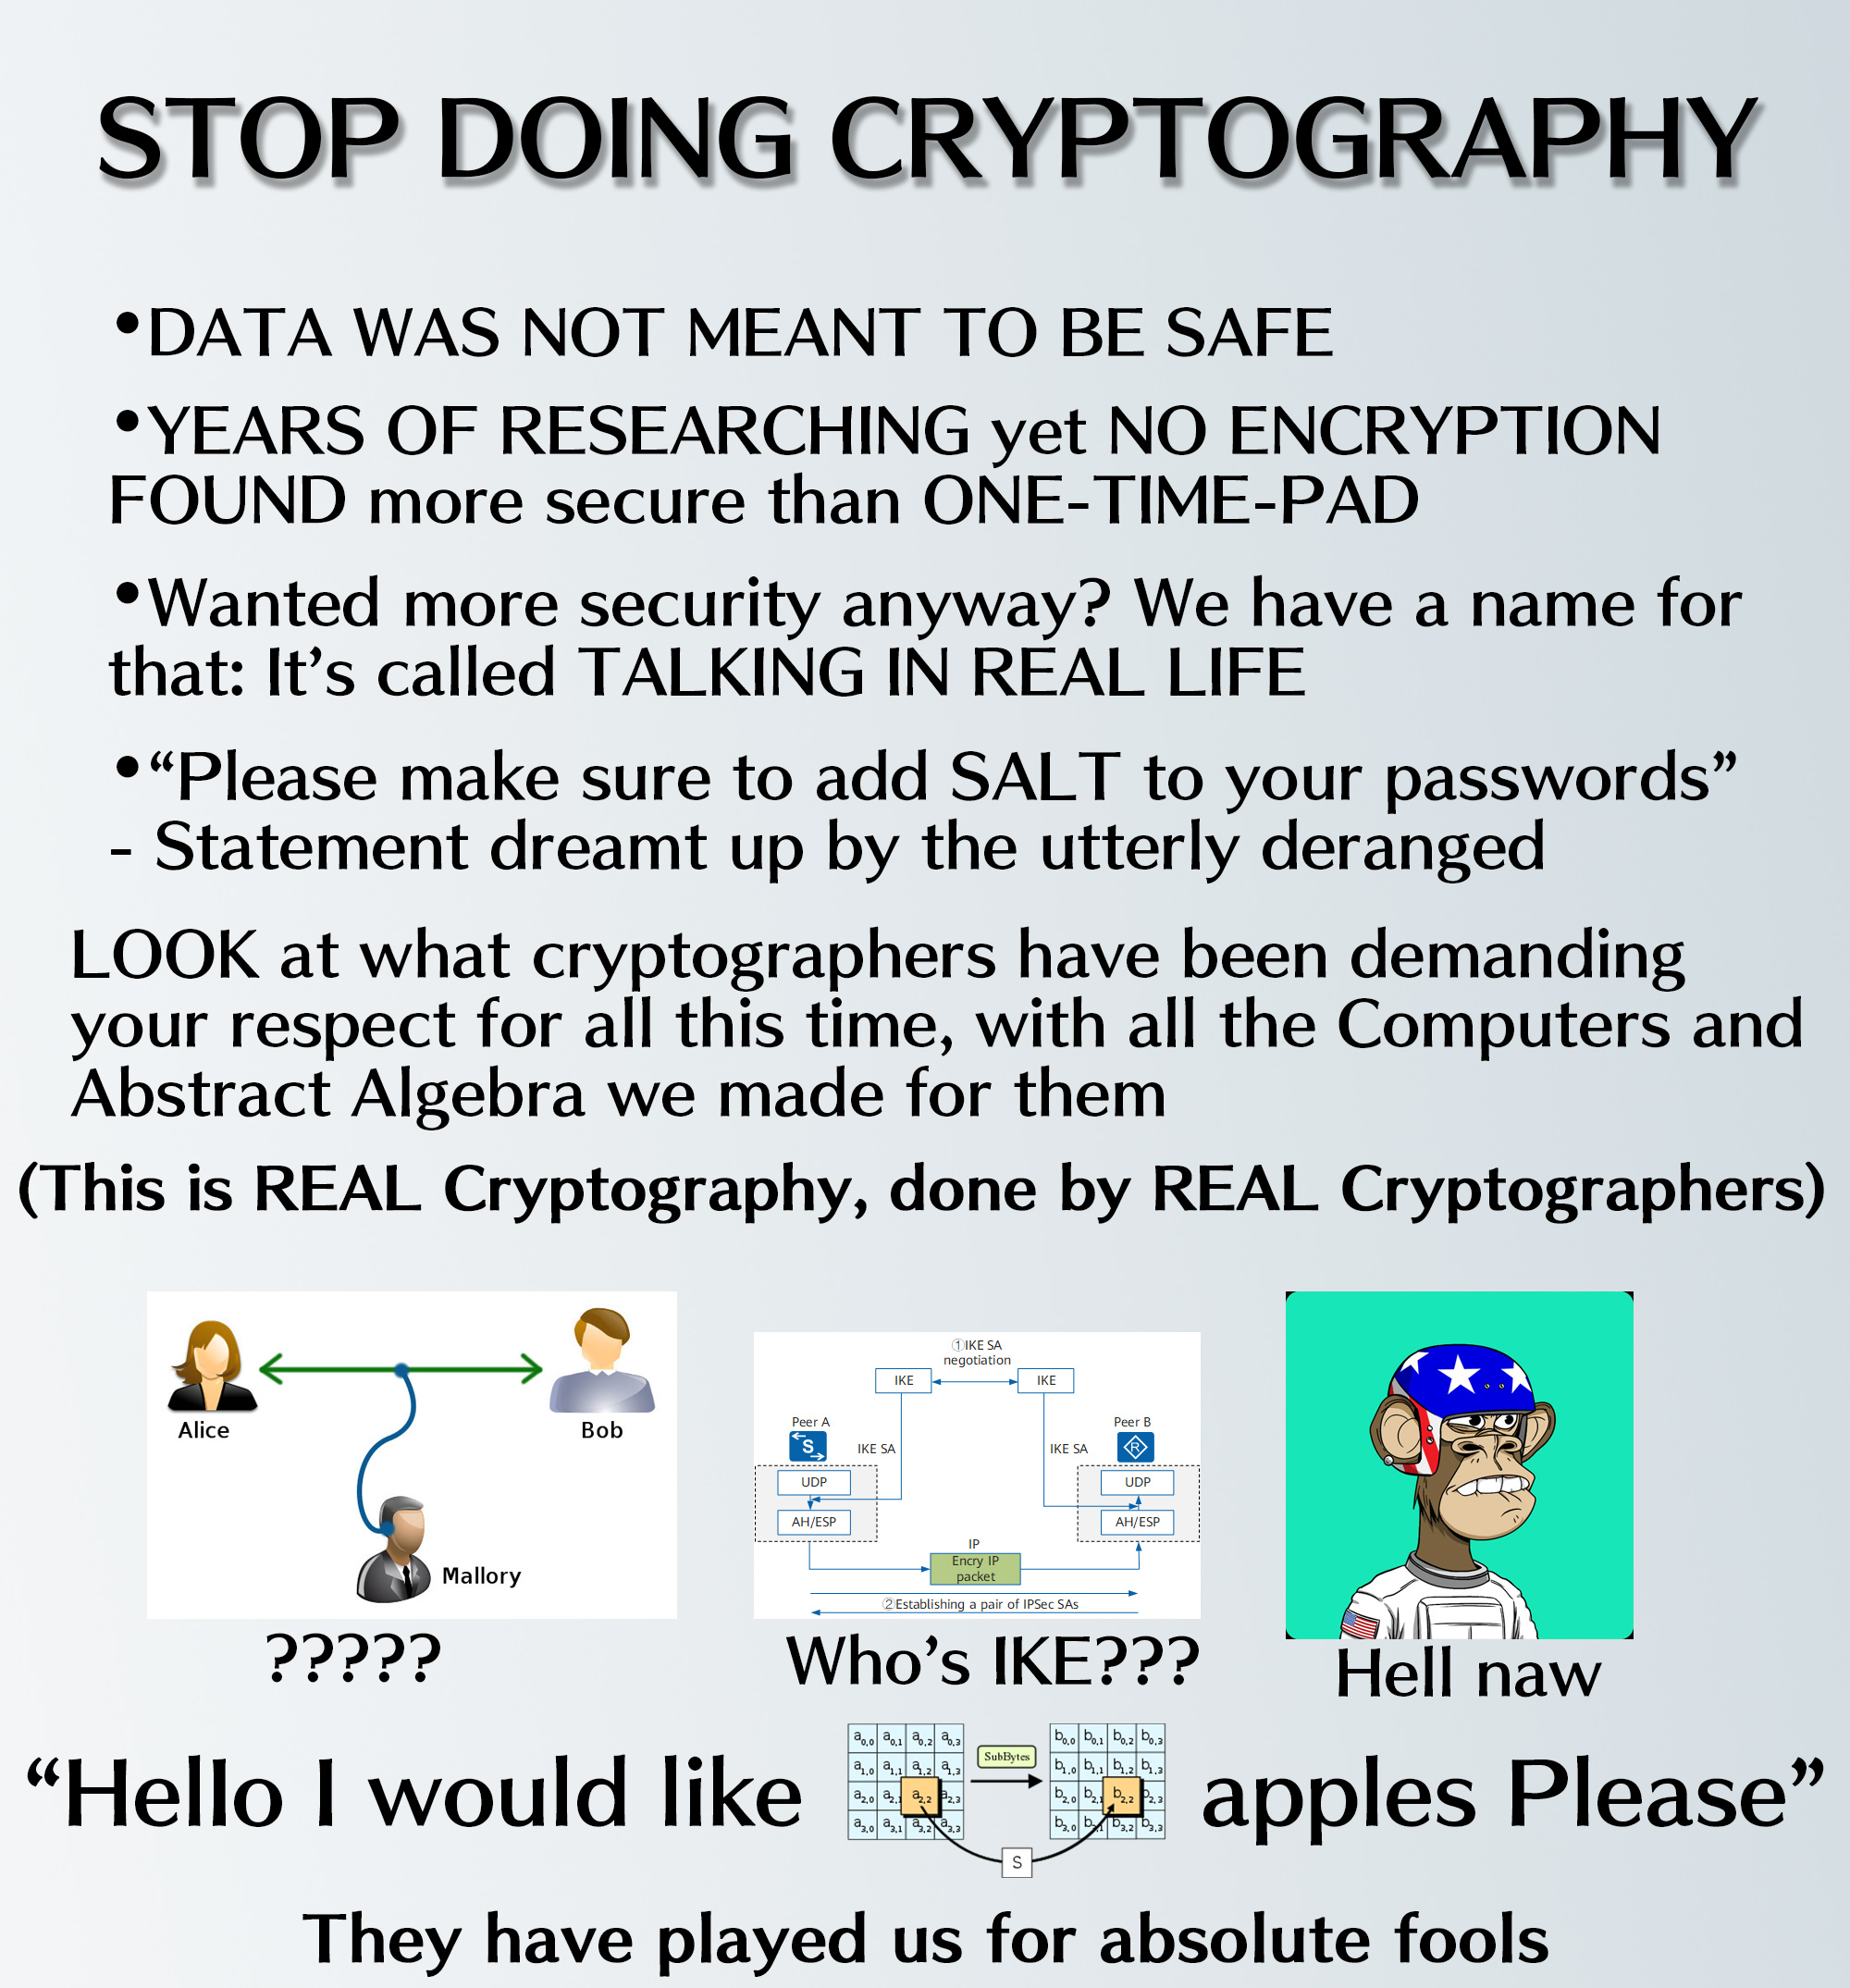
\includegraphics{images/cryptography meme.jpg}

\section{Crypto}\label{crypto}

\subsection{\texorpdfstring{\ul{D}ata \ul{E}ncryption
\ul{S}tandard}{Data Encryption Standard}}\label{data-encryption-standard}

\subsection{\texorpdfstring{\ul{A} \ul{E} \ul{S}}{A E S}}\label{a-e-s}

\begin{itemize}
\tightlist
\item[$\square$]
  Hello
\end{itemize}

\subsection{Hash Functions}\label{hash-functions}

\subsubsection{Block}\label{block}

\section{\texorpdfstring{Docker \faIcon{docker}}{Docker }}\label{docker}

\begin{center}

\includegraphics[width=7cm,height=\textheight]{images/meme_docker.jpg}
\end{center}

\begin{tcolorbox}[enhanced jigsaw, colback=white, leftrule=.75mm, rightrule=.15mm, bottomrule=.15mm, toprule=.15mm, colbacktitle=quarto-callout-important-color!10!white, breakable, opacityback=0, bottomtitle=1mm, titlerule=0mm, toptitle=1mm, title=\textcolor{quarto-callout-important-color}{\faExclamation}\hspace{0.5em}{Wichtig}, coltitle=black, arc=.35mm, left=2mm, colframe=quarto-callout-important-color-frame, opacitybacktitle=0.6]

Bash Befehle via Host sind mit {\color{BrickRed}{\texttt{\textbf{\$}}}}
gekennzeichnet.

\begin{Shaded}
\begin{Highlighting}[]
\ExtensionTok{\$}\NormalTok{ echo }\StringTok{"this happens on WSL or SSH Pi"}
\end{Highlighting}
\end{Shaded}

Bash Befehle in einem Docker Container sind mit
{\color{BrickRed}{\texttt{\textbf{\#}}}} gekennzeichnet.

\begin{Shaded}
\begin{Highlighting}[]
\ExtensionTok{\#}\NormalTok{ echo }\StringTok{"this happens in a Docker container"}
\end{Highlighting}
\end{Shaded}

\end{tcolorbox}

\subsection{Was'n Docka?}\label{wasn-docka}

Kurzgesagt: Docker ``\ul{containerisiert}'' Anwendungen.

Die Idee ist, eine Anwendunge mit der nötigen Konfiguration, Runtime und
Bibliotheken in ein Paket zusammenzustellen und dann als
\textbf{portables} Produkt weitergegeben, verarbeitet, etc. ausgeführt
werden.

Man unterscheidet zwischen \textbf{Image} \& \textbf{Container}

\begin{itemize}
\tightlist
\item
  \textbf{Image} ist eine Vorlage, welche beschreibt, wie ein Container
  aufzubauen ist.
\item
  \textbf{Container} ist die \ul{ausgeführte Instanz eines Images} und
  ist eine \ul{isolierte} Umgebung, welche die entsprechende Prozesse
  ausführt, \textbf{ohne} andere Systeme zu stören.
\end{itemize}

\begin{center}
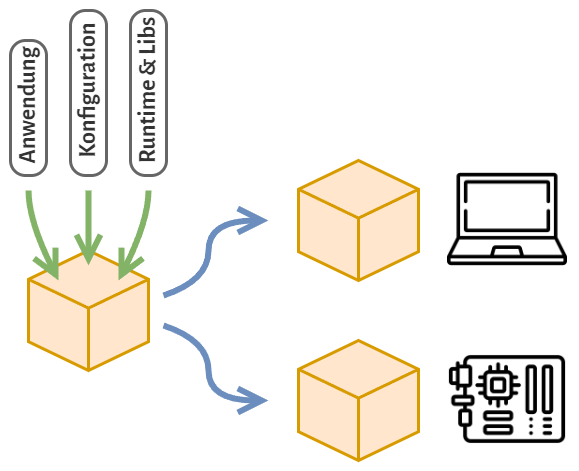
\includegraphics[width=6cm,height=\textheight]{./images/docker/container-distribution.png}
\end{center}

\subsection{Lebenszyklus}\label{lebenszyklus}

Ein Docker-\textbf{Container} kann fünf Zustände annehmen (\ul{Created},
\ul{Running}, \ul{Deleted}, \ul{Stopped} und \ul{Paused}) und kann mit
folgenden Docker-Befehlen gesteuert werden.

\resizebox{\columnwidth}{!}{
  \begin{tikzpicture}[line/.style={-Straight Barb,shorten >=1mm,shorten <=1mm,draw=black, line width=1.5pt}, label/.style={black, fill=white, node font=\bfseries\ttfamily, inner sep=2pt},  node font=\ttfamily]

  \node[circle,fill=YellowGreen,draw=black, inner sep=0, minimum width=1.4cm]   (stateRunning) at (4,6) {running};
  \node[circle,fill=BrickRed!80,draw=black, inner sep=0, minimum width=1.4cm]      (stateStopped) at (4,2) {stopped};
  \node[circle,fill=lightgray,draw=black, inner sep=0, minimum width=1.4cm]     (stateDeleted) at (0,2) {deleted};
  \node[circle,fill=RoyalBlue!30,draw=black, inner sep=0, minimum width=1.4cm]  (stateCreated) at (0,6) {created};
  \node[circle,fill=YellowOrange,draw=black, inner sep=0, minimum width=1.4cm]  (statePaused)  at (8,6) {paused};

  \node (entry1)                at (-3,6)       {};
  \node (entry2)                at (4,8)        {};
  \node [label,left, fill=none] at (3.20,4.75)  {restart};

  \draw [line, OliveGreen, rounded corners=5] (stateRunning) .. controls (3.25,4.75) and (3.25,2.75) .. ([yshift=5mm]stateStopped.center) .. controls (4.75,2.75) and (4.75,4.75) .. (stateRunning);


  \draw [line,YellowGreen]    (stateCreated) edge node[label]        {start}  (stateRunning);
  \draw [line,BrickRed,bend right=4mm] (stateRunning) edge node[label,left=1pt]  {stop}   (stateStopped);
  \draw [line,YellowGreen,bend right=4mm] (stateStopped) edge node[label,right=1pt] {start}  (stateRunning);

  \draw [line,YellowOrange,bend right=4mm] (stateRunning) edge node[label]       {pause}   (statePaused);
  \draw [line,YellowGreen,bend right=4mm] (statePaused)  edge node[label]       {unpause} (stateRunning);
  \draw [line,Gray]                (stateCreated) edge node[label]       {rm}      (stateDeleted);
  \draw [line,Gray]                (stateStopped) edge node[label]       {rm}      (stateDeleted);

  \draw [line,RoyalBlue]                (entry1)       edge node[label]       {create}  (stateCreated);
  \draw [line,YellowGreen]    (entry2)       edge node[label]       {run}     (stateRunning);
  \end{tikzpicture}
}

\subsection{Image Reference Format}\label{image-reference-format}

Standardmässig werden Images wie z.B.
\href{https://registry.hub.docker.com/_/hello-world}{\texttt{hello-world}}
immer vom \href{https://registry.hub.docker.com/}{DockerHub-registry}
heruntergeladen, aber es ist möglich andere \textbf{repos} anzufragen.
Grundsätzlich gilt folgende Struktur:

\begin{center}
\texttt{\textbf{\color{BrickRed}{<repo>}}{\color{Gray}{/}}\textbf{\color{OliveGreen}{<source>}}{\color{Gray}{/}}\textbf{\color{NavyBlue}{<image>}}{\color{Gray}{/}}\textbf{\color{Periwinkle}{<tag>}}}

\end{center}

\begin{itemize}
\tightlist
\item
  \textbf{\texttt{\color{BrickRed}{<repo>}}}: Repository/Content-Host
  (default \texttt{index.docker.io})
\item
  \textbf{\texttt{\color{OliveGreen}{<source>}}} Untergruppe,
  Hauptprojekt, User, Organisation, etc. (default \texttt{library})
\item
  \textbf{\texttt{\color{NavyBlue}{<image>}}} Projekt, wie z.B. eine
  Runtime
\item
  \textbf{\texttt{\color{Periwinkle}{<tag>}}} Version oder Tag des
  Projektes (default \texttt{latest})
\end{itemize}

\begin{Shaded}
\begin{Highlighting}[]
\ExtensionTok{\$}\NormalTok{ docker run }\textbf{\texttt{\color{OliveGreen}{kaohslu}}}/\textbf{\texttt{\color{NavyBlue}{01-demo-img}}}:\textbf{\texttt{\color{Periwinkle}{latest}}}
\end{Highlighting}
\end{Shaded}

\(\rightarrow\) Auf dem offiziellen Repository
\textbf{\texttt{\color{BrickRed}{DockerHub}}} wird unter dem User
\textbf{\texttt{\color{OliveGreen}{kaohslu}}} das Image
\textbf{\texttt{\color{NavyBlue}{01-demo-img}}} der Version
\textbf{\texttt{\color{Periwinkle}{latest}}} heruntergeladen und
gestartet.

\subsection{Volume}\label{volume}

Da die Container voneinander isoliert sind, können diese auch nicht
gegenseitig auf den Speicher zugreifen. Wenn man z.B. Dateien in einen
bestimmten Ordner auf dem Host-Computer abspeichern möchte oder mehrere
Container auf den gleichen Speicher zugreifen lassen, muss dies
\textbf{explizit} angegeben werden.

\begin{center}
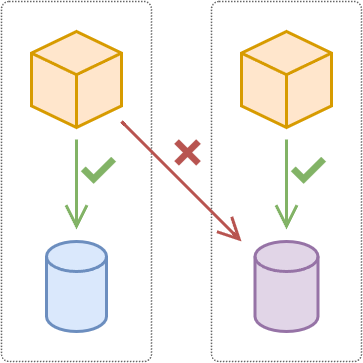
\includegraphics[width=\textwidth,height=4.5cm]{images/docker/container_local_storage.png}
\end{center}

\begin{center}
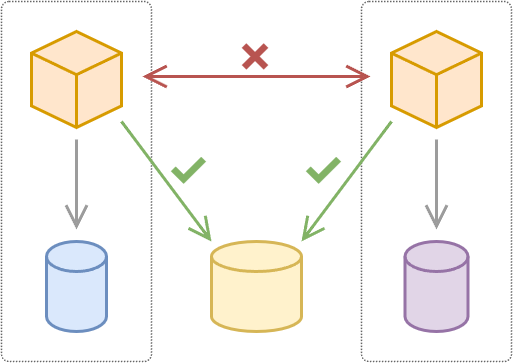
\includegraphics[width=\textwidth,height=4.5cm]{images/docker/container_shared_storage.png}
\end{center}

\section{Safety}\label{safety}

\section{Ada Spark}\label{ada-spark}

\section{Performance}\label{performance}

\subsection{Cache}\label{cache}

\begin{tcolorbox}[enhanced jigsaw, colback=white, leftrule=.75mm, rightrule=.15mm, bottomrule=.15mm, toprule=.15mm, colbacktitle=quarto-callout-note-color!10!white, breakable, opacityback=0, bottomtitle=1mm, titlerule=0mm, toptitle=1mm, title=\textcolor{quarto-callout-note-color}{\faInfo}\hspace{0.5em}{Was Cache?}, coltitle=black, arc=.35mm, left=2mm, colframe=quarto-callout-note-color-frame, opacitybacktitle=0.6]

\end{tcolorbox}

\subsubsection{Trashing}\label{trashing}

\subsubsection{\texorpdfstring{Thrashing /
\href{https://de.wikipedia.org/wiki/Seitenflattern}{Seitenflattern}}{Thrashing / Seitenflattern}}\label{thrashing-seitenflattern}

\subsubsection{Cache Struktur}\label{cache-struktur}

\begin{figure}[H]

\centering{

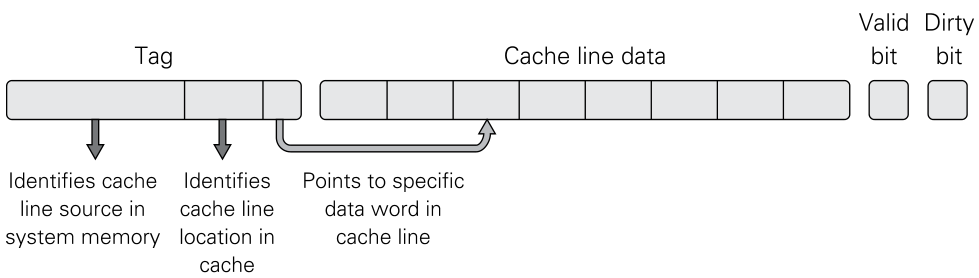
\includegraphics{images/performance/cache-line-structure.png}

}

\caption{\label{fig-performance-cache-line-structure}Struktur einer
Cache-Zeilen}

\end{figure}%

\subsection{GCC Optimization}\label{gcc-optimization}

\texttt{-O0} no optimization \texttt{-O3} all optimization
(\texttt{-O1},\texttt{-O2}) + function inlining and more

\texttt{funroll-loops}

\begin{tcolorbox}[enhanced jigsaw, colback=white, leftrule=.75mm, rightrule=.15mm, bottomrule=.15mm, toprule=.15mm, colbacktitle=quarto-callout-tip-color!10!white, breakable, opacityback=0, bottomtitle=1mm, titlerule=0mm, toptitle=1mm, title=\textcolor{quarto-callout-tip-color}{\faLightbulb}\hspace{0.5em}{Enabling Optimization}, coltitle=black, arc=.35mm, left=2mm, colframe=quarto-callout-tip-color-frame, opacitybacktitle=0.6]

\begin{Shaded}
\begin{Highlighting}[]
\PreprocessorTok{\#pragma GCC optimize ("O0")}
\end{Highlighting}
\end{Shaded}

\end{tcolorbox}

\subsection{}\label{section}

\section{Trends}\label{trends}



\end{document}
